\documentclass[11pt,dvipdfm]{article}

\usepackage{deauthor,times,graphicx}
\graphicspath{{noll/}}

\usepackage{subfig}
\usepackage{listings}
\usepackage{hyperref}


\graphicspath{{./}}










\begin{document}
\title{From the Application to the CPU: Holistic Resource Management for Modern Database Management Systems}
\author{%
{Stefan Noll{\small$~^{\#+*}$}, Norman May{\small$~^{\#}$}, Alexander B\"{o}hm{\small$~^{\#}$}, Jan M\"{u}hlig$~^{+}$, Jens Teubner{\small$~^{+*}$} }
\vspace{1.2mm}\\
\fontsize{10}{10}\selectfont\rmfamily\itshape
$^{\#}$\,SAP SE, Germany\\
\fontsize{9}{9}\selectfont\ttfamily\upshape
\{stefan.noll,norman.may,alexander.boehm\}@sap.com
\vspace{1.6mm}\\
\fontsize{10}{10}\selectfont\itshape
$^{+}$\,Databases and Information Systems Group, TU Dortmund University, Germany\\
\fontsize{9}{9}\selectfont\ttfamily\upshape
jan.muehlig@tu-dortmund.de\\
\fontsize{9}{9}\selectfont\ttfamily\upshape
jens.teubner@cs.tu-dortmund.de
\vspace{1.6mm}\\
\fontsize{10}{10}\selectfont\itshape
$^{*}$\,Informatik Centrum Dortmund e.V., Germany
}
\maketitle

\begin{abstract}
With their capability to perform both high-speed transactional processing and complex analytical workloads on the same dataset and at the same time, Operational Analytics Database Management Systems give enormous flexibility to application developers.
Particularly, they allow for the development of new classes of enterprise applications by giving analytical insights into operational data sets in real time.
From a database system point of view though, these applications are very demanding, as they exhibit a highly diverse combination of  different query workloads with inhomogeneous performance and latency requirements.
In this article, we discuss the practical implications and challenges for database architects and system designers. We propose solutions that---by sharing semantics between the application, the database system, the operating system, and the hardware---allow to manage complex and resource-intensive workloads in an efficient and holistic way.
\end{abstract}



\section{Introduction}
Driven by the idea of enabling both transactional processing as well as real-time analytical query workloads in the context of a single system~\cite{nollhrm19:Plattner:2009:ACA}, a new class of database management systems has emerged, referred to as operational analytics database management systems~\cite{nollhrm19:Boehm:2016:OAD}.
These systems envision to simplify the data management landscape by consolidating multiple, disparate use cases.
Consequently, they allow the creation of novel business applications which seamlessly combine both real-time analytics and transaction processing \cite{nollhrm19:Leukert:2015:TIR}.
From a database system designer's point of view, however, delivering high performance for these modern applications puts up additional challenges because their workload characteristics are highly diverse and demanding.

In particular, static workload management schemes and simple heuristics perform suboptimally considering end-to-end performance~\cite{nollhrm19:Wolf:2014:SUM}.
The reason for this is that even the same query can have different priorities from an application's point of view, depending on the context it is being executed in.
A simple primary-key based lookup operation can be issued, e.g, in the context of a \emph{mission-critical} and time-sensitive OLTP transaction such as the \emph{interactive} data entry by a business user, but also as part of a \emph{non-critical} batch transaction that runs for hours in the \emph{background}.
A complex analytical query can be sent in the context of, e.g., a \emph{scheduled} quarter-end close report (making it rather uncritical from an execution time point of view), but also as part of a \emph{user-driven}, interactive dashboard application where virtually every millisecond counts.

Motivated by these observations, we share the opinion of other researchers that individual hard- and software-solutions throughout the data processing stack fail to address the complex challenges of these systems in isolation~\cite{nollhrm19:Giceva:2013:COD, nollhrm19:Giceva:2017:COS}.
Particularly, we believe that they are best addressed by a holistic approach, and in collaboration between the application, database management system, and the underlying hardware~\cite{nollhrm19:Boehm:2015:NOT}.

\paragraph{Outline.}
This article is structured as follows.
In Section \ref{nollhrm19:sec:hana_wlm}, we discuss how to bridge the semantic gap between the application and the database system.
Communicating additional workload context information and priorities allows the database system to perform prioritization, scheduling, and resource management that is in line with the expectations of the application.
Next, Section \ref{nollhrm19:sec:cpu_cache_partitioning} discusses a similar technique which allows the database system to share semantic information about data access patterns with the underlying hardware (i.e., the processor) by using CPU cache partitioning.
This enables the more efficient utilization of CPU caches, specifically for heterogeneous, highly concurrent workloads.
In Section \ref{nollhrm19:sec:dbms_os}, we highlight different approaches for database management systems to interact with the operating system, e.g., to improve scaling and robustness.
While commercial database systems usually choose to circumvent the OS exploiting detailed workload information, another strategy is bringing the database system and the operating system closer together with a radical co-design.
We conclude the article in Section \ref{nollhrm19:sec:conclusion}.



\section{Workload Management in SAP HANA}
\label{nollhrm19:sec:hana_wlm}

Analytical and transactional workloads do not only have different resource demands, they are also linked to different performance expectations.
\emph{Transactional} workloads are characterized by operations which consume relatively little memory and compute power.
However, they are usually sensitive to lock contention.
Unfortunately, this resource contention leads to fluctuations in statement response times, while applications expect predictable throughput and response time characteristics.
In our experience, customers are willing to sacrifice peak performance in return for better predictability of statement response times.
\emph{Analytical} workloads, on the other hand, typically are demanding regarding CPU and memory consumption.
In particular, single analytical ad-hoc statements may consume excessive amounts of memory or CPU.
This is particularly problematic for operational analytics DBMS when demanding analytical statements take away CPU clock cycles and slow down concurrent transactional workloads~\cite{nollhrm19:Wolf:2014:SUM}.

To balance or prioritize different workloads and to comply with a \emph{service level agreement} (SLA), commercial DBMS usually employ \emph{workload management} to manage resources available to single statements, applications or database users, see~\cite{nollhrm19:Zhang:AWLM:2014} for a good overview.
In SAP HANA, workload management works on a fine-grained level~\cite{nollhrm19:HANA:2018:AdminGuide} because the system is optimized for modern multi-core architectures with extensive multi-threading~\cite{nollhrm19:Psaroudakis:2015:SUC:2824032.2824043}.
Limiting, e.g., the number of working threads or the amount of memory available to the engine, can be managed for entire workloads or individual statements.
While this creates a powerful tuning option for the user, the system has to track and enforce resource consumption in all of its components.
In the following, we briefly present two mechanisms for implementing workload management using the example of SAP HANA: \emph{workload classes} and \emph{admission control}.

\paragraph{Workload Classes.}
In SAP HANA \emph{workload classes} address 1) the requirement of avoiding the excessive resource consumption of single statements and 2) the requirement of isolating the resource demands of different applications, database users, etc.\@
Workload classes are containers of configuration parameters like priority, query timeout, limits of memory consumption, or limits of concurrency per statement or per group of statements.
They are defined in the database catalog and can be applied to all statements of a database connection.
Workload classes depend on context information passed by the client application: session variables, key-value pairs maintained per database connection, e.g., \texttt{APPLICATION="ETL"}.
This context information is matched to a \emph{workload mapping} which defines the set of session variables to consider and the mapping to a workload class.

The example in Listing~\ref{nollhrm19:lst:workload_classes} defines a workload class \texttt{ETLWorkloadClass}.
Statements executed in the context of this workload class may not consume more than $5\,\mathrm{GB}$ of memory and will not use more than one thread.
The corresponding workload mapping \texttt{ETLWorkloadMapping} will apply this workload class if the session variable \texttt{APPLICATION="ETL"} is set in the database connection.
We have confirmed in many customer scenarios that workload classes can significantly help to achieve high performance and robust system behavior.

\begin{lstlisting}[
caption={Simple example of using workload classes in SAP HANA.},
captionpos=b,
label=nollhrm19:lst:workload_classes,
language=SQL,
basicstyle=\ttfamily,
]
CREATE WORKLOAD CLASS "ETLWorkloadClass"
   SET 'STATEMENT MEMORY LIMIT' = '5',
       'STATEMENT THREAD LIMIT' = '1';

CREATE WORKLOAD MAPPING "ETLWorkloadMapping"
       WORKLOAD CLASS "ETLWorkloadClass"
   SET 'APPLICATION NAME' = 'ETL'; 
\end{lstlisting}

\paragraph*{Experimental Results.}
\begin{figure}
\centering
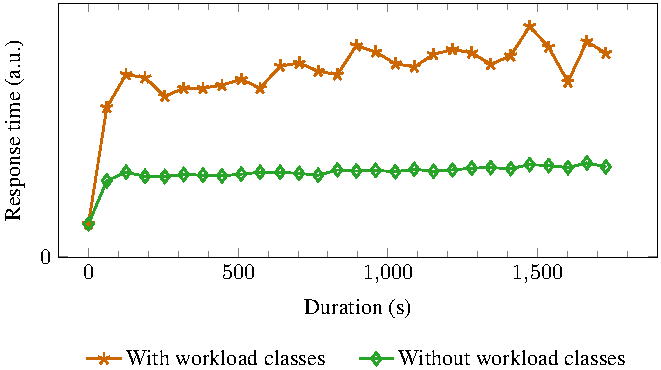
\includegraphics[bb=0 0 317 178]{figs/figure1.pdf}
\caption{Average response time of web requests with and without using workload classes.}
\label{nollhrm19:plt:wlm_jmeter}
\end{figure}
Figure~\ref{nollhrm19:plt:wlm_jmeter} illustrates how workload classes can improve response time of web requests in peak load situations.
We measure the average response time per web request: 
Using JMeter we issue continuously 50 web requests per second.
In addition, we slowly increase analytical and ETL load by adding five queries to each workload every five minutes.
Eventually, we reach a very high system load with close to $100\,\mathrm{\%}$ CPU utilization.
Using workload classes, we limit the ETL and the analytical workload to one thread and $5\,\mathrm{GB}$ of main memory per SQL query (cf. Listing~\ref{nollhrm19:lst:workload_classes}).
Thus, the ETL and analytical load is handled using a best-effort strategy with reduced resource usage.
The results demonstrate that enabling workload class management keeps the average response time of the web requests at a low, predictable value.

\begin{figure}
\centering
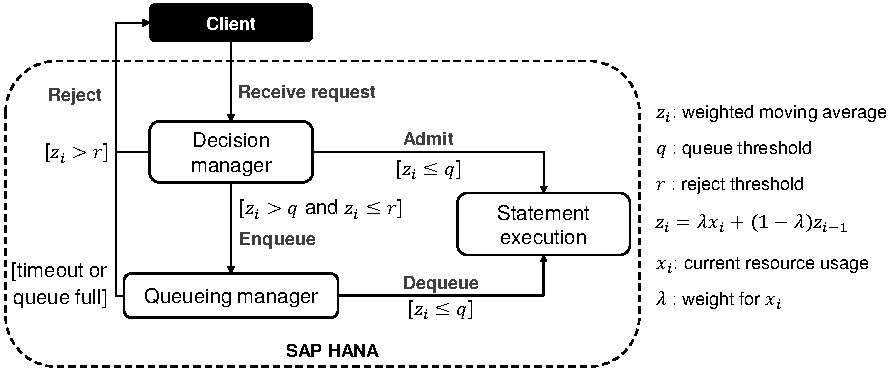
\includegraphics[bb=0 0 427 178]{figs/figure2.pdf}
\caption{Request processing in SAP HANA using admission control.}
\label{nollhrm19:fig:hana_admission_control}
\end{figure}

\paragraph{Admission Control.}
Workload classes influence the resource consumption during execution when a statement was already admitted by the database processes.
However, a reasonably sized system may still experience short peaks in CPU or memory consumption that may result in contention of memory, CPU or latches.
Hence, in SAP HANA we complement workload classes with an \emph{admission control} mechanism.
A schematic overview is depicted in Figure~\ref{nollhrm19:fig:hana_admission_control}.

The admission control mechanism maintains a weighted moving average $z_i$ for all monitored resources of the host such as CPU utilization or total memory consumption.
When SAP HANA receives a new database request, it checks the weighted moving average against thresholds for each resource.
If each $z_i$ is below its corresponding queuing threshold $q$, the statement is admitted for immediate execution.
If the statement cannot be executed immediately, each $z_i$ is checked against its corresponding reject threshold $r$.
If the resource usage is below the reject threshold, the statement is queued; otherwise it is rejected immediately.
SAP HANA periodically checks if the resource consumption has decreased below the queuing threshold.
When this is the case, a batch of requests is fetched from the queue and scheduled for execution.
Database requests may also be rejected when the queue exceeds a configurable size or when the request is queued for too long.

Admission control samples the current resource usage $x_i$ every second.
The value $x_i$ is taken into account with, e.g., a weight of $\lambda = 0.7$.
Note that the sampling interval in combination with the weighted moving average lessens the impact of peak load situations, while the thresholds assure that the system reaches a high load without being overloaded.
In addition, admission control assumes that the client application implements a reasonable strategy to retry rejected database requests.
We could verify in productive setups that admission control helps to avoid contention issues in peak load situations, and that customers profit from a more robust system behavior.

\paragraph*{Conclusion.}
Different workloads have different resource demands and performance characteristics.
To manage hardware resources efficiently or to comply with SLAs of various workloads, commercial systems employ \emph{workload management}.
Using SAP HANA as an example, we present two techniques.
\emph{Workload classes} limit, e.g., the amount of memory or number of threads for an entire workload or an individual statement by enforcing limits across all components of the DBMS.
In addition, \emph{admission control} manages incoming request before they are admitted into the system, monitors CPU and memory consumption, and ultimately accepts or rejects a request to improve response times in peak load scenarios.



\section{CPU Cache Partitioning}
\label{nollhrm19:sec:cpu_cache_partitioning}

Modern microprocessors feature a sophisticated hierarchy of caches to hide the latency of memory access.
However, multiple cores within a processor usually share the same last-level cache (LLC).
We observed that this can hurt performance and predictability, especially in concurrent workloads whenever a query suffers from cache pollution caused by another query running on the same processor: the throughput of cache-sensitive operators may degrade by more than $50\,\mathrm{\%}$~\cite{nollhrm19:Noll:2018}.
In particular, some workloads are highly sensitive to the available amount of CPU cache (e.g., random accesses to a small hash table), contrary to cache-insensitive operations such as a sequential scan of a large memory area.
The good news is that hardware manufacturers allow fine-grained control of cache allocation by offering mechanisms such as Intel's \emph{Cache Allocation Technology} (CAT) \cite{nollhrm19:Intel:2015:CAT:whitepaper}.
By integrating a cache partitioning mechanism, which partitions the cache for individual database operators, into the execution engine of a prototype version of SAP HANA, we were able to improve the overall system performance by up to $38\,\mathrm{\%}$.

\paragraph*{Cache-Sensitivity.}
We analyzed the cache-sensitivity of individual operators using the example of the \emph{column scan} operator, the \emph{aggregation with grouping} operator and the \emph{foreign key join} operator. 
Our results show that \emph{column scans} do not profit from a large LLC.
This observation does not come as a surprise because, by nature, scans read data exactly once from DRAM without re-using it.
\emph{Aggregations}, by contrast, can be highly sensitive to the size of the LLC.
The algorithm that we consider is based on hashing, and is most cache-sensitive whenever the size of the hash tables is comparable to the (configured) LLC size.
Only if the hash table is either very small or very large, cache sensitivity becomes less significant.
Finally, the cache sensitivity of \emph{foreign key joins} heavily depends on the input data, i.e., the cardinality of the primary keys:
If the size of the bit vector used internally is comparable to the size of the cache, the algorithm becomes cache-sensitive.
Otherwise the operator does not profit from a large LLC.

\paragraph*{Cache Partitioning.}
Traditionally, the user has little control over the cache, as it is entirely managed by hardware.
Techniques such as \emph{page coloring}~\cite{nollhrm19:Lee:2009:MMC:1687627.1687670} offer the possibility of partitioning the cache by allocating memory in specific memory pages, known to map to a specific portion of the cache.
But those techniques require significant changes to the OS and the application.
Plus, re-partitioning the cache at runtime requires copying the data~\cite{nollhrm19:4658653, nollhrm19:Zhang:2009:TPP:1519065.1519076}.

\begin{figure}
\centering
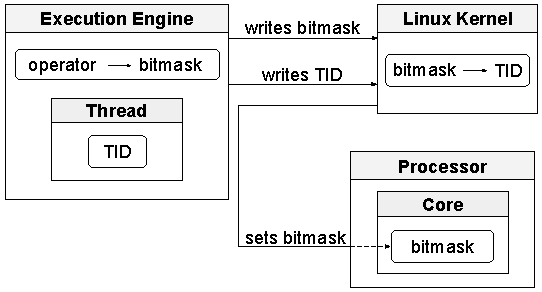
\includegraphics[bb=0 0 260 140]{figs/figure3.pdf}
\caption{Interaction between the execution engine of SAP HANA, the Linux kernel and the processor.}
\label{nollhrm19:fig:hana_cat}
\end{figure}

With the microarchitecture codenamed ``Haswell'' Intel introduced \emph{Cache Allocation Technology} (CAT) \cite{nollhrm19:Intel:2015:CAT:whitepaper} to partition the \emph{last-level cache} of a processor.
We use the Linux kernel interface of CAT (available since version 4.10~\cite{nollhrm19:Intel:2017:CAT:Kernel}) to integrate cache partitioning into the execution engine of a prototype version of SAP HANA\@.
A schematic overview of how we retrofitted cache partitioning into an execution engine is illustrated in Figure \ref{nollhrm19:fig:hana_cat}.

The execution engine of SAP HANA uses a thread pool of worker threads to execute \emph{jobs}~\cite{nollhrm19:Psaroudakis:2015:SUC:2824032.2824043}, e.g., an operator.
We annotate a job with information of its \emph{cache usage}.
The approach is similar to \emph{workload classes}, but its granularity differs.
While \emph{workload classes} annotate entire queries, the cache partitioning mechanism annotates jobs, internal units of work often featuring a distinctive memory access pattern.
Currently, we distinguish between three categories of jobs:
\textit{(i)} jobs which are not cache-sensitive and pollute the cache such as the \emph{column scan};
\textit{(ii)} jobs which are cache-sensitive and profit from the entire cache such as the \emph{aggregation with grouping} operator for most cases; and
\textit{(iii)} jobs such as the \emph{foreign key join} operator which can be both cache-polluting and cache-sensitive depending on the query or data.
By default, a job belongs to \textit{(ii)} to avoid regressions.
During the execution of a job, the engine maps a job to a bitmask and passes the bitmask and the TID of the worker thread to the Linux kernel.
The Linux kernel associates the bitmask with the TID allowing it to update a core's bitmask during thread scheduling.
Integrating cache partitioning into the code base of an industry-strength system, described into more detail in~\cite{nollhrm19:Noll:2018}, requires only a small effort: our actual implementation consists of less than 1000 lines of code.

While we derived the cache partitioning scheme from an experimental analysis, the application of existing characterization methods for \emph{describing} the cache usage pattern of a database operator could be investigated.
For instance, Chou and DeWitt~\cite{nollhrm19:Chou:1985:EBM:1286760.1286772} propose the query locality set model based on the knowledge of various patterns of queries to allocate buffer pool memory efficiently.
Others propose the cache miss ratio as an online model for characterizing workloads or operators~\cite{nollhrm19:Tam:2009:RAL:1508244.1508259, nollhrm19:Manegold:2002:GDC:1287369.1287387, nollhrm19:Zhou:2004:DTP:1024393.1024415}.

\paragraph*{Experimental Results.}
Figure~\ref{nollhrm19:plt:scan_aggregate} illustrates some of our experimental results.
Our evaluation confirms that, e.g., \emph{aggregations} are sensitive to \emph{cache pollution} caused by, e.g., \emph{column scans}.
Aggregations are most sensitive to cache pollution whenever the size of their performance-critical data structures is comparable to the size of the LLC (cf. Figure~\ref{nollhrm19:plt:scan_aggregate}b).
Note that columns in SAP HANA are dictionary-compressed.
A compressed column contains indexes which reference values in a dictionary.
A dictionary is a sorted, unique sequence of the actual domain values.
Because the \emph{aggregation} operator decompresses its input to compute the aggregate, it performs many random accesses to the dictionary of the aggregated column.
Moreover, \emph{aggregations} frequently access hash tables used for grouping.

We observed that the throughput of the \emph{aggregation} query may drop below $60\,\mathrm{\%}$ compared to running isolated in the system.
By utilizing cache partitioning and restricting the \emph{column scan} to $10\,\mathrm{\%}$ of the available LLC, we can improve the throughput of the \emph{aggregation} query by up to $21\,\mathrm{\%}$.
In addition, the \emph{column scan} operator profits from the fact that the \emph{aggregation} operator consumes less memory bandwidth:
The throughput of the \emph{column scan} increases slightly by up to $6\,\mathrm{\%}$, too.
We determine that the overall cache hit ratio increases and that the LLC misses per instruction decrease because the \emph{aggregation} performs fewer accesses to main memory and more accesses to the cache.

While the \emph{column scan} operator always pollutes the cache, other operators such as the \emph{join} operator (not shown here) only cause cache pollution whenever its frequently accessed data structures fit in the L1 or L2 cache~\cite{nollhrm19:Noll:2018}.
In these cases, we can eliminate cache pollution as well and significantly improve performance by restricting the \emph{join} to a small portion of the LLC.
Generally, the search for the ``best'' partitioning in any given situation will depend on accurate \emph{result size estimates}.

\begin{figure}
\centering
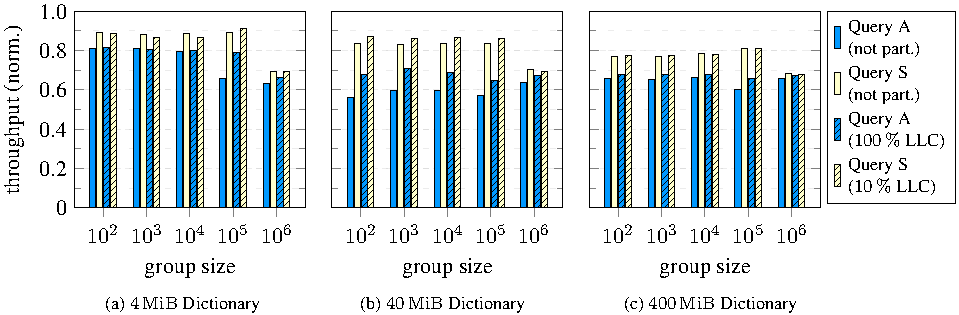
\includegraphics[bb=0 0 460 151]{figs/figure4.pdf}
\caption{%
Throughput of Query~A (\emph{aggregation with grouping}) and Query~S (\emph{column scan}) when executed concurrently (normalized to their throughput when running isolated).
We vary the size of the dictionary of the aggregated column, we vary the number of groups, and we
disable or enable cache partitioning.
}
\label{nollhrm19:plt:scan_aggregate}
\end{figure}

\paragraph{Conclusion.}
In-memory database operators exhibit different performance characteristics depending on the available cache size.
We demonstrate how to integrate a cache partitioning mechanism into the execution engine of an existing DBMS with low expenditure and show in our evaluation that our approach avoids cache pollution and significantly reduces cache misses improving overall system performance.
Ultimately, our results illustrate that integrating cache partitioning into a DBMS engine is worth the effort: it may improve but never degrades performance for arbitrary workloads containing scan-intensive, cache-polluting operators.



\section{Interaction with the OS}
\label{nollhrm19:sec:dbms_os}

The interaction of the database management system with the operation system is crucial for achieving high concurrency, high scalability and robust performance.
While commercial database systems usually choose to circumvent the OS and exploit detailed workload information, another strategy is bringing the database system and the operating system closer together with a radical co-design.
First, we discuss how a database management system may take control of memory management and task scheduling using the example of SAP HANA\@.
Second, we present concepts as well as first experimental results for the bare metal runtime \emph{MxKernel}, a shared platform for implementing crucial components for both the DBMS and the OS. 


\subsection{Bypassing the OS}
\label{snollhrm19:sec:bypassing_os}

Instead of relying on the operating system, SAP HANA takes care of, e.g., the memory management and task scheduling itself---similar to other vendors such as IBM~\cite{nollhrm19:IBM:2004:DB2Memory} and Oracle~\cite{nollhrm19:Oracle:2018:Memory}---to achieve high concurrency, high scalability and robust performance.
In the following, we briefly present how SAP HANA ``bypasses'' the OS using the example of memory management and task scheduling.

\paragraph*{Memory Management.}
In contrast to general-purpose allocators which do not scale to thousands of cores and usually specialize in allocating small blocks, the memory management of SAP HANA is specifically built for the needs of a database system.
It is primarily optimized for high concurrency and scalability in multithreaded and NUMA environments and provides robust performance for the  allocation of different sizes of memory requests and their defragmentation (compaction and garbage collection) during the long operating time of the system (cf.~\cite{nollhrm19:Oukid:2017:MMT:3137628.3137629}).
In addition, the tailor-made implementation supports tracking and monitoring memory operations to provide fine-grained memory usage statistics.
This facilitates limiting the memory consumption globally, per instance, per process, or SQL statement for, e.g., the implementation of workload classes from Section~\ref{nollhrm19:sec:hana_wlm}.
Furthermore, the memory statistics can be used for debugging memory leaks or memory corruption as well as for analyzing performance characteristics related to memory usage.

The memory management pre-allocates memory by requesting chunks of memory (using \texttt{mmap}) from the operating system.
From this point on, the OS is no longer involved.
The cached memory is distributed across different memory pools and completely managed by the database system.
To reduce lock conflicts, each CPU has its own pool.
However, pools can still take memory from other pools.


\paragraph*{Task Scheduling.}

The task scheduling mechanism of SAP HANA utilizes its domain-specific knowledge of database internals to efficiently schedule tasks for highly concurrent, both analytical and transactional workloads.
To mitigate the problem of blocking tasks in transactional workloads, the task scheduler dynamically adapts the number of threads in the self-managed thread pool and prioritizes short-running OLTP queries.
At the same time, the scheduler makes use of a dynamic concurrency hint for analytical workloads, which results in a lower number of tasks for OLAP queries avoiding synchronization, communication and scheduling costs~\cite{nollhrm19:PsaroudakisSMA13}.
In general, the task scheduler relies on the scheduler of the Linux kernel to map threads to cores, but it, e.g., manages the thread placement to NUMA nodes explicitly and supports task stealing to deal with under-utilization~\cite{nollhrm19:Psaroudakis:2016:AND:3015274.3015275}.





\subsection{DB/OS Co-Design}
Most DBMS such as SAP HANA implement, e.g., their own memory management or task scheduling to achieve high concurrency, high scalability as well as robust performance.
Bypassing the OS comes at a price, however.
First, the DBMS re-implements features already existing in the OS.
This means that program code may be duplicated, which in return creates unnecessary maintenance and development costs.
In addition, with the OS and the DBMS having their own implementations it becomes increasingly difficult to share information.
Hence, the DBMS might have detailed information about its workloads, but at the same time it lacks the comprehensive hardware and system information available to the OS and vice versa.
Second, bypassing the OS works best if the DBMS is the only application.
However, as soon as the DBMS is co-running with another application on the same machine, e.g., in a cloud scenario or an on-premise infrastructure, dynamically managing a machine's hardware resources becomes very difficult.

A solution could be the introduction of a central component to which each application as well as the OS communicate their resource demands.
Such a component could then possess detailed information about each of the applications' workloads running on the OS \emph{and} about the OS itself.
Consequently, a radical \emph{co-design} of OS and DBMS (as well as other applications) could address the problem of dynamic resource management on a shared machine.
A first step into this direction is the bare-metal platform \emph{MxKernel}, which we introduce in the following.

\paragraph*{Architecture of MxKernel.}
Usually, DBMS are built on top of an underlying OS which is used to abstract the machine's hardware such as CPU architectures or complex memory hierarchies.
This abstraction can result in the loss of information relevant to the DBMS.
For example, applications running on top of the OS have less knowledge about parallel executed applications, the load factor of the machine and the actual hardware structure.
Using external libraries like \texttt{libnuma}~\cite{nollhrm19:kleen2005numa} might help to gain additional hardware information such as local and remote memory areas or the NUMA distribution of CPU cores.
But the use is more like a crutch and does not solve the problem holistically.
It remains, e.g, difficult to explore and utilize cache hierarchies or topology structures of various modern hardware~\cite{nollhrm19:Giceva:2013:COD}.

\begin{figure}
\centering
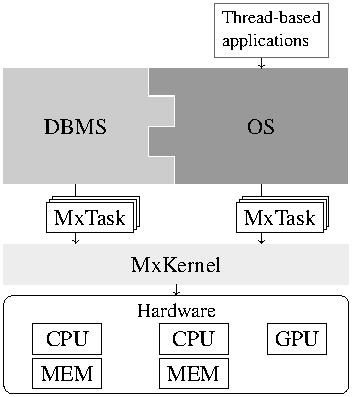
\includegraphics[bb=0 0 169 190]{figs/figure5.pdf}
\caption{%
MxKernel provides a small basis layer for managing shared hardware resources between all applications running on a shared machine, including, e.g., the OS and the DBMS.
}
\label{nollhrm19:plt:mxkernel}
\end{figure}

A first step towards solving these problems in a holistic way is the bare-metal platform MxKernel.
Figure \ref{nollhrm19:plt:mxkernel} depicts an overview of the architecture.
The platform's core is a basis layer, which enables to run all applications as well as the OS side by side.
Note that running an OS is optional.
At the same time, MxKernel provides a detailed view of the hardware and an interface to which an application can communicate its requirements regarding hardware resources or performance expectations.

In particular, it implements services for hardware compatibility and a mechanism for control flow execution.
Moreover, its architecture allows, e.g., the OS and the DBMS to share data structures and algorithms such as B-Trees, which can be used for primary key indexing by the DBMS or for implementing a file system by the OS.

\paragraph*{MxTasks.}

The platform MxKernel introduces \emph{MxTasks} to abstract from and to create an interface to the control flow execution.
MxTasks describe small units of work representing a more lightweight alternative to POSIX Threads.
They are executed atomically by implementing a run-to-completion semantic.
Usually, MxTasks feature only a small sequence of instructions.
As a result, their runtime, memory accesses, and resource requirements are easier to predict and to define than threads.
In addition, MxTasks can be coupled with precise metadata about, e.g., its memory access patterns, its accessed data structures and its preferred NUMA region.
Thus, by annotating \emph{MxTasks} with workload information we employ the same concept of sharing semantics between application, OS, DBMS, and hardware as discussed for \emph{workload classes} in Section~\ref{nollhrm19:sec:hana_wlm} or for \emph{jobs} in Section~\ref{nollhrm19:sec:cpu_cache_partitioning}.

MxKernel creates an execution plan that synchronizes MxTasks for shared-resource accesses and optimizes them for cache and NUMA locality.
Thus, MxKernel functions as a central component for resource management which receives (workload) information in the form of MxTasks with metadata.
Its execution framework then tries to fulfill the requirements of all applications as well as possible.
Applications running on top of an (optional) OS, however, can still choose to use threads instead of MxTasks for compatibility reasons.

Furthermore, MxTasks represent a way to exploit heterogeneous systems by providing different implementations for distinct processing units such as GPUs or CPUs.
Based on system load and the runtime property of a MxTask, MxKernel could then choose the most suitable available hardware for execution.

\paragraph*{Experimental Results.}
As a first use case, we evaluated an index data structure based on the B\textsuperscript{link}-tree~\cite{nollhrm19:Lehman:1981:ELC:319628.319663}.
We implement the insert algorithm described by Lehman and Yao~\cite{nollhrm19:Lehman:1981:ELC:319628.319663}.
However, we modify it to support MxTasks: We spawn a new task for each traversal of a node.
This means that we create a task for looking up the child node to traverse next.
When a task finally finds the matching leaf node, we insert the new value.

While concurrent POSIX Threads accessing the same node of the B\textsuperscript{link}-tree have to be protected using latches, MxTasks benefit from the run-to-completion semantic:
Mapping the traversal of a tree node to a specific processor core ensures that only one task accesses a node at a time.
In addition, we benefit from cache locality because one core accesses the same data structure multiple times.

\begin{figure}
\centering
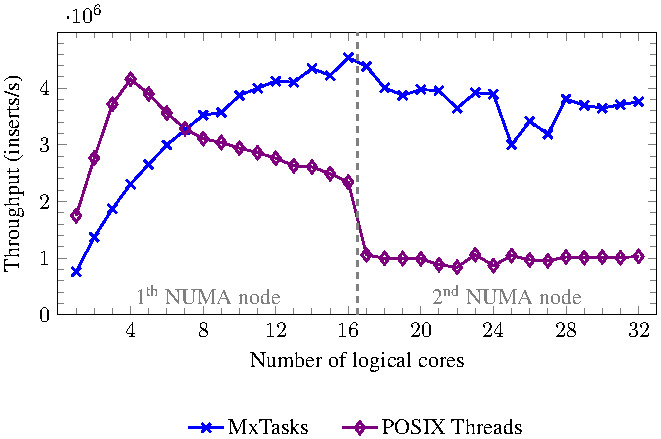
\includegraphics[bb=0 0 317 211]{figs/figure6.pdf}
\caption{Throughput of insert operations into a B\textsuperscript{link}-tree. While the throughput drops down when using more than four POSIX Threads, the throughput stagnates when using MxTasks from the second NUMA region.}
\label{nollhrm19:fig:blinktree:results}
\end{figure}

We consider two different implementations of the B\textsuperscript{link}-tree: a version based on POSIX Threads executed on Linux, and a version based on MxTasks running on MxKernel.
The workload consists of $16 \cdot 10^6$ insert operations using unique key-value pairs.
We execute the experiment on a system with two Intel Xeon E5-2690 processors with 8 CPU cores each, and simultaneous multithreading enabled.

The results illustrated in Figure \ref{nollhrm19:fig:blinktree:results} show that while the thread-based version exhibits a higher throughput until using eight threads, the throughput starts dropping after using four threads.
We explain the differences with the latch contention of the thread version:
Every node has to be protected by a latch to prevent inconsistencies.
MxTasks, on the other hand, have no need to use latches.
Every node of the B\textsuperscript{link}-tree is assigned to one of the cores and every MxTask accessing a node will be executed on the mapped core without suspension.

In addition, we notice that the throughput degrades slightly after using cores from the second NUMA node.
We attribute this to the increased overhead of cache coherency.
For managing MxTasks and tracking their execution state, we use a wait-free queue for every core.
Pushing MxTasks from a queue of one core to the queue of another core, triggers the cache coherency mechanism of the processor which costs additional execution time.
This effect occurs as soon as another NUMA node is involved.
Note that the throughput of the thread-based version, on the other hand, drops significantly with more than 16 cores.


\paragraph*{Conclusion.}
The interaction between DBMS and OS are crucial for creating high-performance systems.
We briefly present how a commercial system such as SAP HANA bypasses the OS and implements, e.g., its own memory management and task scheduling to guarantee robust performance and scaling by exploiting domain-specific knowledge, or to track and to enforce the consumption of hardware resources.
Another strategy is the co-design of DBMS and OS.
As a first step towards this goal, we introduce the bare-metal platform \emph{MxKernel}.
On top of it, the DBMS and the OS run side by side with an interface to communicate their hardware and runtime requirements to.
In return, MxKernel manages hardware resources exclusively.



\section{Conclusion}
\label{nollhrm19:sec:conclusion}

Operational analytics database management systems with the capability to perform both high-speed transactional processing and complex analytical workloads on the same dataset and at the same time, impose new challenges and practical implications for system designers.
In this article, we discussed several solutions that allow to manage these resource-intensive workloads in an efficient and holistic way.
In particular, we explicitly share workload information between application, OS, DBMS, and hardware which allows us to manage resources efficiently and to improve performance and predictability.

By sharing context information between the application and the DBMS, systems can implement an application-aware resource management and quality of service features.
SAP HANA employs \emph{workload classes} for limiting the resource consumption of queries issued by individual applications.
In addition, we presented its \emph{admission control} mechanism to manage the amount of requests the system handles at a given time in order to avoid contention in peak load situations.

By sharing cache usage information between the DBMS and the hardware, we implement a mechanism that \emph{dynamically partitions} the \emph{cache} per individual operator.
We demonstrated that this may improve the overall throughput of highly concurrent workloads, where we restrict the cache usage of scan-intensive operators and increase the cache capacity for cache-sensitive operators.

Finally, we discussed how the database system interacts with the operating system.
While DBMS traditionally take control over individual features of the OS and implement, e.g., a custom memory management or task scheduling, other research directions explore their co-design.
In particular, we presented the bare-metal platform \emph{MxKernel}.
On top of it, the DBMS and the OS run side by side and communicate their hardware and runtime requirements to the platform.
In return, MxKernel takes care of managing all hardware resources.

\section*{Acknowledgments}
This work was supported by DFG, Deutsche Forschungsgemeinschaft, grant number TE 1117/2-1.




\begin{thebibliography}{10}
\itemsep=1pt
\begin{small}
\bibitem{nollhrm19:Plattner:2009:ACA}
H.~Plattner. \newblock A Common Database Approach for OLTP and OLAP Using an In-Memory Column Database. \newblock \emph{SIGMOD}, 2009, pp. 1--2.

\bibitem{nollhrm19:Boehm:2016:OAD}
A.~B{\"{o}}hm, J.~Dittrich, N.~Mukherjee, I.~Pandis, and R.~Sen. \newblock Operational Analytics Data Management Systems. \newblock \emph{VLDB}, vol.~9, no.~13, pp.
1601--1604, 2016.

\bibitem{nollhrm19:Leukert:2015:TIR}
H.~Plattner and B.~Leukert. \newblock The In-Memory Revolution: How SAP HANA Enables Business of the Future. \newblock Springer, 2015.

\bibitem{nollhrm19:Wolf:2014:SUM}
I.~Psaroudakis, F.~Wolf, N.~May, T.~Neumann, A.~B{\"{o}}hm, A.~Ailamaki, and
K.~Sattler. \newblock Scaling up Mixed Workloads: a Battle of Data Freshness, Flexibility, and Scheduling. \newblock \emph{TPCTC}, 2014, pp. 97--112.

\bibitem{nollhrm19:Giceva:2013:COD}
J.~Giceva, T.~Salomie, A.~Sch{\"{u}}pbach, G.~Alonso, and T.~Roscoe. \newblock COD: Database / Operating System Co-Design. \newblock \emph{CIDR}, 2013.

\bibitem{nollhrm19:Giceva:2017:COS}
K.~Kara, J.~Giceva, and G.~Alonso. \newblock FPGA-based Data Partitioning. \newblock \emph{SIGMOD}, 2017, pp. 433--445.

\bibitem{nollhrm19:Boehm:2015:NOT}
A.~B{\"{o}}hm. \newblock Novel Optimization Techniques for Modern Database Environments. \newblock \emph{BTW}, 2015, pp. 23--24.

\bibitem{nollhrm19:Zhang:AWLM:2014}
M.~Zhang. \newblock Autonomic Workload Management for Database Management Systems. \newblock \emph{Ph.D. thesis}, Queen's University, 2014.

\bibitem{nollhrm19:HANA:2018:AdminGuide}
\mbox{SAP SE}.\hspace{1mm}\mbox{SAP HANA Administration Guide}.\hspace{1mm}\url{https://help.sap.com/viewer/6b94445c94ae495c83a19646e7c3fd56/2.0.03/en-US}, 2018.

\bibitem{nollhrm19:Psaroudakis:2015:SUC:2824032.2824043}
I.~Psaroudakis, T.~Scheuer, N.~May, A.~Sellami, and A.~Ailamaki. \newblock Scaling Up Concurrent Main-Memory Column-Store Scans: Towards Adaptive NUMA-aware Data and Task Placement. \newblock \emph{VLDB}, vol.~8, no.~12, pp. 1442--1453,
2015.

\bibitem{nollhrm19:Noll:2018}
S.~Noll, J.~Teubner, N.~May, and A.~B\"{o}hm. \newblock Accelerating Concurrent Workloads with CPU Cache Partitioning. \newblock \emph{ICDE}, 2018,
pp. 437--448.

\bibitem{nollhrm19:Intel:2015:CAT:whitepaper}
Intel Corporation. \newblock Improving Real-Time Performance by Utilizing Cache Allocation Technology. \newblock \emph{White paper}, 2015.

\bibitem{nollhrm19:Lee:2009:MMC:1687627.1687670}
R.~Lee, X.~Ding, F.~Chen, Q.~Lu, and X.~Zhang. \newblock MCC-DB: Minimizing Cache Conflicts in Multi-core Processors for Databases. \newblock \emph{VLDB},
vol.~2, no.~1, pp. 373--384, 2009.

\bibitem{nollhrm19:4658653}
J.~Lin, Q.~Lu, X.~Ding, Z.~Zhang, X.~Zhang, and P.~Sadayappan. \newblock Gaining Insights into Multicore Cache Partitioning: Bridging the Gap Between Simulation and Real Systems. \newblock \emph{HPCA}, IEEE Computer Society, 2008, pp. 367--378.

\bibitem{nollhrm19:Zhang:2009:TPP:1519065.1519076}
X.~Zhang, S.~Dwarkadas, and K.~Shen. \newblock Towards Practical Page Coloring-based Multicore Cache Management. \newblock \emph{EuroSys}, ACM, 2009, pp. 89--102.

\bibitem{nollhrm19:Intel:2017:CAT:Kernel}
Intel Corporation. \newblock User Interface for Resource Allocation in Intel Resource Director Technology. \newblock Documentation of the Linux Kernel, \url{https://www.kernel.org/doc/Documentation/x86/intel_rdt_ui.txt}, 2017.

\bibitem{nollhrm19:Chou:1985:EBM:1286760.1286772}
H.-T. Chou and D.~J. DeWitt. \newblock An Evaluation of Buffer Management Strategies for Relational Database Systems. \newblock \emph{VLDB}, 1985, pp. 127--141.

\bibitem{nollhrm19:Tam:2009:RAL:1508244.1508259}
D.~K. Tam, R.~Azimi, L.~B. Soares, and M.~Stumm. \newblock RapidMRC: Approximating L2 Miss Rate Curves on Commodity Systems for Online Optimizations. \newblock \emph{ASPLOS}, ACM, 2009, pp.
121--132.

\bibitem{nollhrm19:Manegold:2002:GDC:1287369.1287387}
S.~Manegold, P.~Boncz, and M.~L. Kersten. \newblock Generic Database Cost Models for Hierarchical Memory Systems. \newblock \emph{VLDB}, 2002, pp. 191--202.

\bibitem{nollhrm19:Zhou:2004:DTP:1024393.1024415}
P.~Zhou, V.~Pandey, J.~Sundaresan, A.~Raghuraman, Y.~Zhou, and S.~Kumar. \newblock Dynamic Tracking of Page Miss Ratio Curve for Memory Management. \newblock \emph{ASPLOS}, ACM, 2004, pp.
177--188.

\bibitem{nollhrm19:IBM:2004:DB2Memory}
IBM. \newblock The DB2 UDB memory model -- How DB2 uses memory. \newblock \url{https://www.ibm.com/developerworks/data/library/techarticle/dm-0406qi/}, 2018.

\bibitem{nollhrm19:Oracle:2018:Memory}
Oracle. \newblock Database Administrator’s Guide -- Managing Memory. \newblock \url{https://docs.oracle.com/database/121/ADMIN/memory.htm}, 2018.

\bibitem{nollhrm19:Oukid:2017:MMT:3137628.3137629}
I.~Oukid, D.~Booss, A.~Lespinasse, W.~Lehner, T.~Willhalm, and G.~Gomes. \newblock Memory Management Techniques for Large-Scale. Persistent-Main-Memory Systems. \newblock \emph{VLDB}, vol.~10, no.~11, pp. 1166--1177, 2017.

\bibitem{nollhrm19:PsaroudakisSMA13}
I.~Psaroudakis, T.~Scheuer, N.~May, and A.~Ailamaki. \newblock Task Scheduling for Highly Concurrent Analytical and Transactional Main-Memory Workloads. \newblock \emph{ADMS}, 2013, pp. 36--45.

\bibitem{nollhrm19:Psaroudakis:2016:AND:3015274.3015275}
I.~Psaroudakis, T.~Scheuer, N.~May, A.~Sellami, and A.~Ailamaki. \newblock Adaptive NUMA-aware Data Placement and Task Scheduling for Analytical Workloads in Main-Memory Column-Stores. \newblock \emph{VLDB}, vol.~10, no.~2, pp. 37--48, 2016.

\bibitem{nollhrm19:kleen2005numa}
A.~Kleen. \newblock A NUMA API for Linux. \newblock \emph{White paper}, SUSE Labs, 2004.

\bibitem{nollhrm19:Lehman:1981:ELC:319628.319663}
P.~L. Lehman and S.~B. Yao. \newblock Efficient Locking for Concurrent Operations on B-Trees. \newblock \emph{ACM Trans. Database Syst.}, vol.~6, no.~4, pp. 650--670, 1981.
\end{small}
\end{thebibliography}

\end{document}
